\documentclass[runningheads]{llncs}
\def\shownotes{1}
\def\notesinmargins{0}

\usepackage{fancyvrb}
\usepackage{mathtools,color,xcolor,hyperref,graphicx,wrapfig,listings,array,xspace}
\usepackage{caption}
\usepackage{subcaption}
\usepackage{tikz}
\usetikzlibrary{arrows}

\usepackage{amsfonts}
\usepackage{xcolor}
\usepackage{alltt}

\usepackage{listings}
\usepackage{xcolor}

\definecolor{codegreen}{rgb}{0,0.6,0}
\definecolor{codegray}{rgb}{0.5,0.5,0.5}
\definecolor{codepurple}{rgb}{0.58,0,0.82}
\definecolor{backcolour}{rgb}{0.95,0.95,0.92}

\lstdefinestyle{mystyle}{
    backgroundcolor=\color{backcolour},
    commentstyle=\color{codegreen},
    keywordstyle=\color{magenta},
    numberstyle=\tiny\color{codegray},
    stringstyle=\color{codepurple},
    basicstyle=\scriptsize \ttfamily, %\footnotesize, %or \small
    breakatwhitespace=false,
    breaklines=true,
    captionpos=b,
    keepspaces=true,
    numbers=left,
    numbersep=5pt,
    showspaces=false,
    showstringspaces=false,
    showtabs=false,
    tabsize=2
}

\lstset{style=mystyle}

% Compensate for fbox sep:
\newcommand\Hi[2][lightgray]{%
    \hspace*{-\fboxsep}%
    \colorbox{#1}{#2}%
    \hspace*{-\fboxsep}%
}

\renewcommand{\lstlistingname}{Contract}% Listing -> Contract
\renewcommand{\lstlistlistingname}{List of \lstlistingname s}% List of Listings -> List of Contracts

\ifnum\shownotes=1
\ifnum\notesinmargins=1
\newcommand{\authnote}[2]{\marginpar{\parbox{\marginparwidth}{\small %
\textsf{#1 {\textcolor{blue}{notes: #2}}}}}%
\textcolor{blue}{\textbf{\dag}}}
\else
\newcommand{\authnote}[2]{
    \textsf{#1 \textcolor{blue}{: #2}}}
\fi
\else
\newcommand{\authnote}[2]{}
\fi

\newcommand{\snote}[1]{{\authnote{\textcolor{yellow}{Scalahub notes}}{#1}}}
\newcommand{\knote}[1]{{\authnote{\textcolor{green}{kushti notes}}{#1}}}


\newcommand{\ret}{\mathsf{ret}}
\newcommand{\new}{\mathsf{new}}
\newcommand{\hnew}{h_\mathsf{new}}
\newcommand{\old}{\mathsf{old}}
\newcommand{\op}{\mathsf{op}}
\newcommand{\verifier}{\mathcal{V}}
\newcommand{\prover}{\mathcal{P}}
\newcommand{\key}{\mathsf{key}}
\newcommand{\nextkey}{\mathsf{nextKey}}
\newcommand{\node}{\mathsf{t}}
\newcommand{\parent}{\mathsf{p}}
\newcommand{\leaf}{\mathsf{f}}
\newcommand{\vl}{\mathsf{value}}
\newcommand{\balance}{\mathsf{balance}}
\newcommand{\lft}{\mathsf{left}}
\newcommand{\rgt}{\mathsf{right}}
\newcommand{\lbl}{\mathsf{label}}
\newcommand{\rand}{\stackrel{R}{\leftarrow}}
\newcommand{\direction}{\mathsf{d}}
\newcommand{\oppositedirection}{\bar{\mathsf{d}}}
\newcommand{\found}{\mathsf{found}}
\newcommand{\mypar}[1]{\smallskip\noindent\textbf{#1.}\ \ \ }
\newcommand{\ignore}[1]{}

\newcommand{\ergoscript}{ErgoScript\xspace}
\newcommand{\ergomix}{ErgoMix\xspace}
\newcommand{\zerocoin}{Zerocoin\xspace}
\newcommand{\zerojoin}{Zerojoin\xspace}

\newcommand{\lst}[1]{\text{\lstinline[basicstyle={\ttfamily}]$#1$}}

\newcommand{\andnode}{\ensuremath{\mathsf{AND}}}
\newcommand{\ornode}{\ensuremath{\mathsf{OR}}}
\newcommand{\tnode}{\ensuremath{\mathsf{THRESHOLD}}}

\newcommand{\GF}{\ensuremath{\mathrm{GF}}}

\AtBeginDocument{\renewcommand*{\thelstlisting}{\arabic{lstlisting}}}

\begin{document}

\newcommand{\algname}{Sigmajoin\xspace}
\title{\algname: Outsourceable \zerojoin}

\maketitle

\begin{abstract}

We present \algname, a privacy protocol for UTXO-based
blockchains. \algname is an enhancement of \zerojoin, which is also a privacy protocol.
Like \zerojoin, our protocol is non-interactive in the sense that Alice does not need to be online when Bob mixes their coins.
However, \zerojoin requires a party to be online for remixing. \algname is even more non-interactive than \zerojoin because
once parties add  their coins to the pool, they don't need to be online for remixing, which can be carried out by a trustless service.
Thus, while our protocol retains all the features of \zerojoin, it additionally provides {\em outsourceability}. Similar to \zerojoin, our protocol also uses proofs of knowledge of Diffie-Hellman tuples, where we prove equivalence of exponents in two pairs of group elements. The privacy of our protocol also depends on the hardness of the Decisional-Diffie-Hellman (DDH) problem. Like \zerojoin, our protocol can also be implemented using \ergoscript.
\end{abstract}

\section{Introduction}
\label{intro}


Privacy enhancing techniques in UTXO-based blockchains generally fall into two categories. The first is obscuring the input-output relationships such as in \zerocoin~\cite{zerocoin}, Composite Signatures (CS)~\cite{composite}, CoinJoin~\cite{coinjoin} and \zerojoin~\cite{zerojoin}. The second is hiding the amounts being transferred, such as in Confidential Transactions~\cite{ct}. Some solutions such as Zcash~\cite{zcash,zcash1}, Quisquis~\cite{quisquis} and MimbleWimble (MW)~\cite{mw} combine both approaches.

In this work, we describe \algname, yet another privacy enhancing protocol based on the former approach of obscuring input-output relationships. Our protocol is motivated from \zerojoin~\cite{zerojoin} to overcome some of its limitations:

\begin{enumerate}
    \item {\em Mix more than 2 boxes}: In \zerojoin, we can mix only two boxes at a time and it will be good to have a solution that works for more than 2 boxes
    \item {\em Make it outsourceable}: In \zerojoin, Bob can mix a box of Alice without interaction. However, to remix a full-mix box, one must be online. Requiring participants to be continuously online makes the protocol {\em non-outsourceable}, and thereby less usable. This is also a problem with CoinJoin~\cite{coinjoin}. It is preferable to remix a box without the owner's intervention.
    \item {\em Do away with half-mix boxes}: In \zerojoin, we need to create a half-mix box when playing Alice's role for remixing, while Bob's role can be played directly using the full-mix box. Thus, half-mix boxes are `bloat'~\cite{zerojoin} and it will be better to directly work with full-mix boxes.
\end{enumerate}

\section{Background}
\subsection{Notation}

Let $G$ be a cyclic group of prime order $q$ where the Decisional-Diffie-Hellman (DDH) problem is hard and let $g, h, u, v$ be generators of $G$.
In the following, {\em proveDlog$(g, u)$} refers to a zero-knowledge proof of knowledge of discrete logarithm of $u$ to base $g$ and {\em proveDHTuple$(g, h, u, v)$} refers to a zero-knowledge proof of equality of the following two discrete logarithms: $u$ to base $g$ and $v$ to base $h$. The proofs are described in Appendices~\ref{provedlog} and~\ref{provedhtuple} respectively, and are implemented using {\em Sigma protocols}~\cite{zerojoin,CDS94}.
For any two sigma protocols $\sigma_1$ and $\sigma_2$, the symbol $\sigma_2 \textsf{ OR } \sigma_2$ refers to the zero-knowledge OR described in Appendix~\ref{sigmaor}, that is, a proof of knowledge of one of them without revealing which~\cite{CDS94}.

\subsection{Basic idea}
The following describes the high level idea for mixing two boxes at a time. The same idea can be trivially extended to mix three, four, etc boxes.

\zerojoin~\cite{zerojoin} consists of two types of boxes: a {\em half-mix} box protected by a script of type {\em proveDlog$(*, *)$} and a {\em full-mix} box having a script of type {\em proveDlog$(*, *)$} \textsf{OR} {\em proveDHTuple$(*, *, *, *)$}. This makes the two boxes incompatible and we cannot remix as Alice without creating a half-mix box first. Note that we can still remix as Bob directly, but that is only possible if there are half-mix boxes available.
%, because of which we cannot remix a full-mix box directly while playing Alice’s role; we must first create a half-mix box.
Additionally, the half-mix box is a kind of ``bloat'' and it is preferable to operate with full-mix boxes only (called just ``mix'' boxes).

The idea of \algname is to start with two boxes having a script of type {\em proveDlog$(*, *)$} and have the mix also generate two boxes of type {\em proveDlog$(*, *)$}. In particular, a mix box has two registers $a, b$ containing elements of $G$ and the owner has to prove the statement: {\em proveDlog$(a, b)$}.
Since we have only one type of box in \algname, we will have only one type of participant, called Alice.

\section{\algname Protocol}

Privacy in \algname is provided via a pool of coins (boxes). People add coins to the pool and later withdraw them in a manner that hides the links between the entry and exit boxes.
A box in the pool, called a {\em mix-box}, is defined as follows:
\begin{itemize}
    \item It has two registers labeled $a, b$ containing elements of $G$.
    \item It is protected by the {\em mix-script} given in Section~\ref{smart-contract}. One part of the script allows spending the box freely by proving the statement: {\em proveDlog$(a,b)$}. The other part allows anyone to spend the box only in a restricted manner, that is, if it is used in mixing as per Section~\ref{mix}.
\end{itemize}

The protocol, illustrated in Figure~\ref{fig:sigmajoin}, consists of three operations:

\begin{enumerate}
    \item {\em Deposit}: Anyone can deposit coins in {\em fixed} denominations to the pool.
    \item {\em Withdraw}: This allows anyone to withdraw their coins from the pool.
    \item {\em Mix}: Anyone (the ``mixer'') can spend any two coins from the pool, thereby ``mixing'' them, and then add them back as two indistinguishable coins that preserve the original owners. The mixer need not be the owner of one of the inputs.
    A box is mixed several times before it is finally withdrawn.
\end{enumerate}

\begin{figure}[h]
    \centering
    \begin{subfigure}{.8\textwidth}
        \centering
        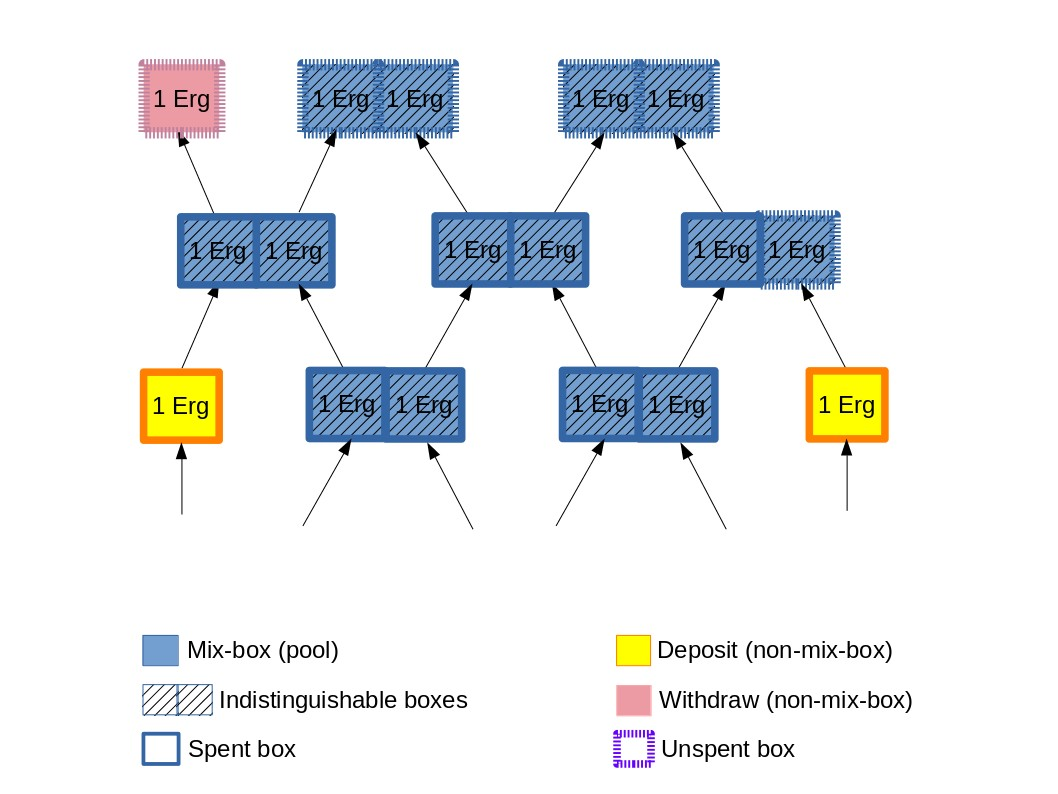
\includegraphics[width=\linewidth]{Sigmajoin.jpg}
    \end{subfigure}%
    \caption{\algname protocol}
    \label{fig:sigmajoin}
\end{figure}

\subsection{Deposit and Withdraw}

Let $g$ be a fixed generator of $G$. To deposit a box to the pool, Alice selects secret $x\rand \mathbb{Z}_q$ and creates a box protected by the mix-script with registers $(a, b)$ containing $(g, g^x)$. Alice can withdraw her box at any time using the secret $x$.

\subsection{Mix}
\label{mix}

A mix is done by selecting two mix-boxes from the pool and spending them in a transaction that generates two identical-looking mix-boxes. An output is generated by applying the following transformation each input.

\begin{enumerate}
\item Generate secret $y \rand \mathbb{Z}_q$ and apply the transformation $(a, b) \leftarrow (a ^y, b ^y)$. In other words, register $a$ (resp. $b$) of the new box is computed by raising register $a$ (resp. $b$) of the old box to power $y$. The transformation preserves the secret exponent relationship between $a$ and $b$, ensuring the owner's ability to spend the box anytime. This is called {\em re-randomising} the public key.
\item To ensure that the mix is done correctly, that is, both registers are raised to the same power, the mixer must additionally prove the following statement.

Let $(a_0, b_0)$ and $(a_1, b_1)$ be the registers of the first and second output respectively. Then the mixer must prove:
$$\text{\em proveDHTuple$(a, b, a_0, b_0)\textsf{ OR }$proveDHTuple$(a, b, a_1, b_1)$}$$

\item We additionally need to ensure that $y \neq 0$, which can be done by requiring that $a_0 \neq b_0$ and $a_1 \neq b_1$.

\end{enumerate}

\subsection{Ergo and ErgoScript}

We implement our protocol in ErgoScript, the scripting language of the Ergo blockchain~\cite{ergo,tutorial}. We use Ergo because it has the {\em proveDHTuple} protocol built-in, is UTXO based and supports advanced scripts at context level C3~\cite{bypassing}. ErgoScript is a strict subset of the Scala language. It allows accessing the inputs and outputs of the transaction and specifying arbitrary constraints on them.
ErgoScript has a restricted form of {\em proveDlog$(*, *)$}, namely {\em proveDlog$(g, *)$}, where $g$ is fixed.
This is denoted as {\em proveDlog$(*)$}. We can overcome this limitation using the rule {\em proveDlog$(a, b)$} = {\em proveDHTuple$(a, a, b, b)$}.

Data in Ergo boxes is stored in up to 10 registers labeled R0 to R9, out of which R0 to R3 are reserved by the protocol and the remaining are for user-defined values~\cite{tutorial}. We use the following mapping: $a \rightarrow$ R4 and $b \rightarrow$ R5.

The object to be proved, the content of a script is called a {\em proposition}, which consists of either one or two {\em statements}. A statement evaluates to \texttt{true} or \texttt{false} during
runtime. When two statements are present, they must be joined using logical \em{And} or \em{Or}. A box can be spent when its script evaluates to \texttt{true}.

Statements are of two types: {\em primitive} and {\em compound}. A compound statement is made by joining two (primitive or compound) statements using {\em And} or {\em Or}. A primitive statement can be either a {\en crypto-statement} (such as \texttt{proveDlog} or \texttt{proveDHTuple}) or a predicate on the context (such as \texttt{a <= b}).

A crypto-statement requires a proof using which it evaluates to either \texttt{true} or \texttt{false} depending on whether the proof is valid or not.
Thus, the output of every statement is always a boolean value, and the logical operations are meaningful.
Whenever two crypto-statements are to be joined using {\em Or}, they are done using zero-knowledge (see  Appendix~\ref{sigmaor}).
Whenever a crypto-statement is to be joined with a predicate, the predicate is first evaluated and the crypto-statement is evaluated lazily. In other words, a statement like \texttt{proveDlog(...) \&\& false} is considered equivalent to the predicate \texttt{false} and statements like \texttt{proveDlog(...) \&\& true} or \texttt{proveDlog(...) || false} are considered equivalent to \texttt{proveDlog(...)}. The final statement is then just combination of pure crypto-statements joined using {\em Or} and {\em And}.

\subsection{Smart Contract}
\label{smart-contract}

The contract of a mix box is given below in ErgoScript
\begin{lstlisting}[language=Scala,caption={Mix-script},label=mixScript]
val a = SELF.R4[GroupElement].get     // current base for dLog
val b = SELF.R5[GroupElement].get
val owner = proveDHTuple(a, a, b, b)  // = proveDlog(a, b)
val mix = {
  val out0 = OUTPUTS(0)   // first output
  val out1 = OUTPUTS(1)   // second output
  val a0 = out0.R4[GroupElement].get  // register a of first output
  val a1 = out1.R4[GroupElement].get  // register a of second output
  val b0 = out0.R5[GroupElement].get  // register b of first output
  val b1 = out1.R5[GroupElement].get  // register b of second output
  val validOuts = out0.propositionBytes == SELF.propositionBytes &&
  out1.propositionBytes == SELF.propositionBytes &&
  out0.value == SELF.value &&
  out1.value == SELF.value &&
  a0 != b0 && // rule out point at infinity ToDo: explain more
  a1 != b1    // rule out point at infinity

  // at least one of the outputs has the right relationship between R4, R5
  val validAB = proveDHTuple(a, b, a0, b0) || proveDHTuple(a, b, a1, b1)

  validAB && validOuts
}

mix || owner
\end{lstlisting}

\subsection{Analysis}

With regards to security, no one should be able to spend Alice's box other than for mixing ({\em theft-prevention}) and Alice should always be able to spend her box ({\em spendability}). Both are guaranteed by ensuring the exponent relationship between $a, b$ of at least one of the box in the mix, and additionally requiring $a, b$ to be not O (the point at infinity). With regards to privacy, no outsider should be able to guess with an advantage, which output corresponds to which input. For $i \in \{0, 1\}$, the transformation of $(a_i, b_i)$ from inputs to outputs using secret $y_i$ can be written as:
$(a_i, b_i) \leftarrow ({a_i}^{y_i}, {b_i}^{y_i})$. If the DDH problem is hard then the output distributions $(a_0, b_0), (a_1, b_1)$ are indistinguishable.

\section{Extensions}

Here we discuss various enhancements to the basic protocol presented above.

\subsection{Outsourceability}

Unlike \zerojoin, an interesting possibility with \algname is that of {\em outsourcing} the mix process, where the mixing is done in a trustless manner by third parties called mixers. In this approach, shown in Figure~\ref{fig:joiner}, multiple mixers operate on the same pool. The mixers are {\em non-custodial} in the sense that while they have the ability to deanonymize users, they don't have the ability to steal funds.

%We note that other protocols with a similar structure, such as \zerojoin and CoinJoin do not support this.

\begin{figure}[ht]
\centering
\begin{subfigure}{0.8\textwidth}
\centering
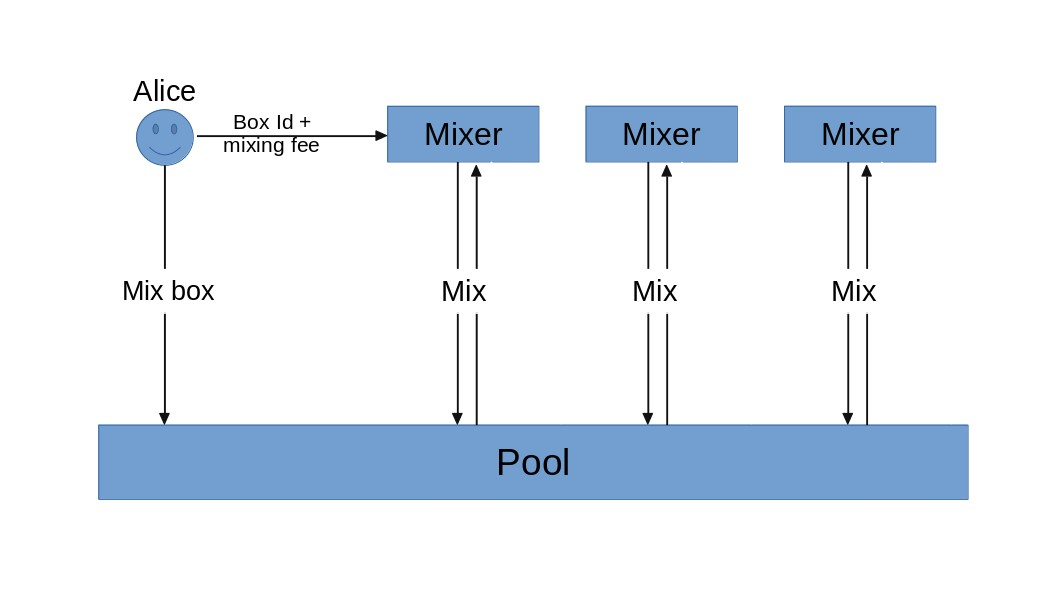
\includegraphics[width=\linewidth]{Joiner.jpg}
\end{subfigure}%
\caption{Outsourced fee}
\label{fig:joiner}
\end{figure}

Alice adds her mix-box to the pool and sends the box id (a globally unique identifier) to a mixer along with some {\em mixing fee}. The mixer then proceeds to mix Alice's box several times as determined by the mixing fee.
One problem with this approach is that the mixer may lose track of Alice's box if someone else mixes her box in between. In order to prevent this, we can put a time-lock that prevents anyone else but the mixer from spending the box before a certain time. The modified contract is given below:

\begin{lstlisting}[language=Scala,caption={Mix-script with Outsourceability},label=mixScript]
val a = SELF.R4[GroupElement].get  // current base for dLog
val b = SELF.R5[GroupElement].get
val m = SELF.R6[GroupElement].get  // public key of the mixer or dummy value
val h = SELF.R7[Int].get // height at which box was created
val lockTime = 5 // number of blocks for which box is time-locked
val owner = proveDHTuple(a, a, b, b)  // = proveDlog(a, b)
val mixer = proveDlog(m)              // = proveDlog(g, m), g is fixed
val timeOut = HEIGHT > h + lockTime
val mix = {
  val out0 = OUTPUTS(0)   // first output
  val out1 = OUTPUTS(1)   // second output
  val a0 = out0.R4[GroupElement].get  // register a of first output
  val a1 = out1.R4[GroupElement].get  // register a of second output
  val b0 = out0.R5[GroupElement].get  // register b of first output
  val b1 = out1.R5[GroupElement].get  // register b of second output
  val m0 = out0.R6[GroupElement].get  // just access group element
  val m1 = out1.R6[GroupElement].get  // just access group element
  val h0 = out0.R7[Int].get  // height at which first output is created
  val h1 = out1.R7[Int].get  // height at which second output is created
  val validOuts = out0.propositionBytes == SELF.propositionBytes &&
  out1.propositionBytes == SELF.propositionBytes &&
  out0.value == SELF.value &&
  out1.value == SELF.value &&
  a0 != b0 && // rule out point at infinity
  a1 != b1 && // rule out point at infinity
  h0 <= HEIGHT && // ensure that h0 is not too high
  h1 <= HEIGHT    // ensure that h1 is not too high

  // at least one output has the right relationship between R4, R5
  val validAB = proveDHTuple(a, b, a0, b0) || proveDHTuple(a, b, a1, b1)

  validAB && validOuts && (mixer || timeOut)
}

owner || mix
\end{lstlisting}

To determine the mixing fee, assume that Alice wants to mix her box $n$ times (example $n = 10$). At each mix, there is onex extra box created. In order to ensure that Alice's box is not identified by outsiders, the mixer must process every such extra box as if it were Alice's box. Thus, about $2^{n+1}$ mix transactions must be generated by the mixer, and in the worst case, the mixing fee should cover as many transactions. In reality, the mixer would combine Alice's and other's mixes, and so not all mixes will be just for Alice.

\subsection{Stealth Withdraw}
\label{stealth-withdraw}
A mix box can either be used for (re)mixing or be withdrawn. When a mix box is reused in mixing, there is no {\em transfer-of-value} as the box owner remains the same. On the other hand, a withdraw is necessary for transfer-of-value. However, we note that the original protocol also allows transfers-of-value transactions that look like mix transactions and it becomes infeasible for an outsider to distinguish the two types.

This is possible because the owner has the ability to spend the box anytime because of the final condition \texttt{owner || mix}. The owner can do so in a manner where the final transaction looks like a mix transaction but is actually not.
This can be done by ensuring that \texttt{validOuts} and \texttt{timeOut} in Contract~2 is true.
The final contract then reduces to \texttt{owner || validAB} joined using a zero-knowledge proof.
This allows the owner to create a transaction that resembles a mix transaction but does not require ownership to be preserved.

A transfer of value using this technique is a {\em stealth withdraw} since it cannot be distinguished from a mix transaction.
Using the idea of stealth withdraw, we don't ever have to withdraw from the pool;
all transactions happen within the pool, thereby increasing the privacy further.
Note that while a mix can be outsourced, a stealth withdraw cannot.

\section{Outsourced Fee}

One of the challenging problems in mix protocols is that of mining fee. Since the fee has to be paid in a manner that does not reveal the source of funds, the parties cannot pay it using arbitrary boxes owned by them. Additionally, since the mix has to preserve the value, the fee cannot be paid using the tokens being mixed. There are two approaches to handling mining fee in such scenarios.
\begin{enumerate}
\item {\em Embedded}: The fee must be embedded in the mix boxes themselves. This is the primary approach is followed in \ergomix~\cite{zerojoin} via {\em mixing tokens}.
\item {\em External}: The fee is paid by a third party who has no relationship with the participants. An example is the {\em altruistic fee} approach described in \cite{zerojoin}.
In this work, we propose {\em outsourced fee}, another external approach.
\end{enumerate}

While the embedded fee approaches of~\cite{zerojoin} will also work with \algname,
outsourceability allows us to design a much simpler external approach where the fee is paid by the mixer.
We call this {\em Outsourced Fee}. Referring to Figure~\ref{fig:joiner},
each mixer maintains its own set of unspent boxes for covering mining fee, which we call {\em funding boxes}.
\footnote{
For a stealth withdraw, which cannot be outsourced, the simplest way is for the owner to privately purchase the private key of a funding box from a mixer.}

There are two roles in the system and anyone can take one or the other role:
\begin{enumerate}
\item Mixers (privacy providers): Who provide the service for a profit in Ergs by performing the mix on behalf of users.
\item Users (Privacy seekers): Who want privacy of their tokens without ever losing control of them
\end{enumerate}

The main requirement of a mixer is to keep a lot of funding boxes in advance to pay mining fee.
The funding boxes should ideally be unrelated to the boxes being mixed. However, a mixer can use boxes where it received payment for its service as long as it selects such boxes randomly. We also discuss ways to make on-chain payment to a mixer without leaking information about the mixer or the box.

Although a user {\em can} perform a mix, (because the smart contract does not differentiate the two users), the privacy of our solution
relies on the fact that only mixers perform a mix. A user performing its own mix can leak information via the source of fee.
A user is free to mix random boxes from the pool, thereby following the ``altruistic fee'' approach. However, it makes more sense for such users to take the role of a mixer.


\subsection{Contract}

We will use the following modified contract in mix boxes. The contract has some differences from the earlier version:
\begin{enumerate}
\item For efficiency, instead of storing creation height in R7, we will use the context variable \texttt{creationInfo.\_1}, which already has the same value~\cite{ergo-data-model}.
We will store some other information in R7 instead.
\item Instead of identifying a mixer using a single group element, we will use two elements, denoted $m, n$ in the contract. This is to allow the possibility of stealth payments~\cite{stealth-payments} to the mixer.
\item In addition to just the primary token (Erg), we require {\em all} tokens of the output boxes to be identical and same as the input tokens.
\end{enumerate}


\begin{lstlisting}[language=Scala,caption={Mix-script with Stealth Outsourceability},label=mixScript]
val a = SELF.R4[GroupElement].get  // public key of owner (base for dLog)
val b = SELF.R5[GroupElement].get  // public key of owner (base ^ secret)
val m = SELF.R6[GroupElement].get  // public key of the mixer (base)
val n = SELF.R7[GroupElement].get  // public key of the mixer (base ^ secret)
// We are using two elements (m, n) to represent mixer, rather than one
// because this allows "stealth" locking a box to a mixer
// (i.e., without revealing the mixer identity)
// So mixer will publish public key (u, v), two group elements.
// In order to lock the box to the mixer, Alice will set (m, n) = (u^r, v^r)
// for secret and random r

val h = SELF.creationInfo._1 // height at which box was created

val lockTime = 50 // number of blocks for which box is time-locked

val owner = proveDHTuple(a, a, b, b)  // = proveDlog(a, b)
val mixer = proveDHTuple(m, m, n, n)  // = proveDlog(m, n)

val timeOut = HEIGHT > h + lockTime

val mix = {
  val out0 = OUTPUTS(0)   // first output
  val out1 = OUTPUTS(1)   // second output

  val a0 = out0.R4[GroupElement].get  // register a of first output
  val a1 = out1.R4[GroupElement].get  // register a of second output
  val b0 = out0.R5[GroupElement].get  // register b of first output
  val b1 = out1.R5[GroupElement].get  // register b of second output

  val m0 = out0.R6[GroupElement].get  // access group element (not used)
  val m1 = out1.R6[GroupElement].get  // access group element (not used)
  val n0 = out0.R7[GroupElement].get  // access group element (not used)
  val n1 = out1.R7[GroupElement].get  // access group element (not used)

  val h0 = out0.creationInfo._1  // height at which first output is created
  val h1 = out1.creationInfo._1  // height at which second output is created

  // ensure outputs have same script as this box and have the same value
  val validOuts = out0.propositionBytes == SELF.propositionBytes &&
  out1.propositionBytes == SELF.propositionBytes &&
  out0.value == SELF.value &&
  out1.value == SELF.value &&
  out0.tokens == SELF.tokens &&
  out1.tokens == SELF.tokens &&
  a0 != b0 && // rule out point at infinity
  a1 != b1 && // rule out point at infinity
  h0 <= HEIGHT && // ensure that h0 is not too high
  h1 <= HEIGHT // ensure that h1 is not too high

  // at least one of the outputs has the right relationship between R4, R5
  val validAB = proveDHTuple(a, b, a0, b0) || proveDHTuple(a, b, a1, b1)

  validAB && validOuts && (mixer || timeOut)
}

owner || mix
\end{lstlisting}

The contract implements the following rules:
\begin{enumerate}
\item Allows a 3rd party to `lock' the box so that only that party can mix it for a certain time (\texttt{lockTime}).
\item Allows a 3rd party to mix the box as long as it does not violate rule 1 (i.e., after \texttt{lockTime} is over).
\item Allows the owner to always spend the box, overriding any conditions imposed by above rules.

\end{enumerate}

In our solution, spending via rule 1 will be done by a mixer, one who has been explicitly paid to mix the tokens contained in the box.
Spending via rule 2 will be done by a mixer who has not been paid to mix this box, but is doing so to enhance privacy of their mix transaction.
In order to maintain privacy, the order of boxes will not determine whether it is being spent via rule 1 or 2.

Since spending the box requires mining fee, usually, anyone who spends via 1 or 2 will only do so if they get some benefit.
There are two possible benefits:
\begin{enumerate}
\item A mixer will earn profit as service fee paid via a different (possibly offchain) channel.
\item A mixer will spend in order to gain privacy for a box it wants to mix.
\end{enumerate}

\subsection{Stealth Payments}

Another useful primitive is {\em stealth payments}~\cite{stealth-payments} (not to be confused with stealth withdraw of Section~\ref{stealth-withdraw}).
To receive a stealth payment, first generate a random group element $h$ and a secret $x$. Then compute $k = h^x$ and publish $(h, k)$.
A stealth payment is made by generating a box protected by the script \texttt{proveDHTuple}$(h^r, h^r, k^r, k^r)$.
This is considered `stealth' because given $(h^r, k^r)$, it is not possible to deduce $(h, k)$
assuming that the DDH problem is hard.

In reality, we will actually store $(h^r, k^r)$ in (R4, R5)
and make the script \texttt{proveDHTuple}(R4, R4, R5, R5).
Anyone expecting stealth payments to secret $x$ must scan all boxes protected by the above script and select those where R5$ = $R4$ ^ x$.


Mixing fee can be paid via stealth payments to the mixer's public key $(m, n)$ (stored in (R6, R7) of the mix box).
In other words, the payment will be made to a box locked with the script \texttt{proveDHTuple}$(m^r, m^r, n^r, n^r)$ for a secret $r$.
Note that the initial value of $(m, n)$ stored in the user's box should itself be the randomized version of the mixer's public key
(as we did above with $r$), to hide the mixer to which the box is locked to. The mixer will then do a similar randomization at each mix.

The payment box can additionally store the user's box id encrypted using, say, El Gamal with the same public key $(m, n)$.

\subsection{Mixer Strategy}

We define the strategy from a mixer's point of view. Let $P$ be the set of mix-boxes that are free (i.e., not locked to any mixer) and let $L$ be the set of boxes that are locked to this mixer. Thus, $P$ and $L$ are disjoint. We will assume that $P$ always has an unlimited supply of boxes. We can incentivize users to keep their boxes in $P$ as discussed later. The mixer can be bootstrapped once $L$ has at least one box. The suggested strategy for the mixer is to always operate on boxes in $L$ only

\subsubsection{Operation}

Once a mixer is bootstrapped (i.e., $L$ is sufficiently large), it can perform the actual mixes as follows.
\begin{enumerate}
\item Pick two boxes from $L$ uniformly.
\item Mix them and add them back to $L$ (i.e., lock them again).
\item Repeat and keep track of boxes in order to decide when a box is sufficiently mixed.
\item For boxes where the lock is about to expire (i.e., those about to be removed from $L$),
spend them again in a mix transaction with other active boxes to ensure $L$ always has enough boxes.
If $L$ already has enough boxes, the mixer can let such boxes be unlocked using a random strategy.

\end{enumerate}

\subsubsection{Bootstrapping}

Whenever the number of boxes in $L$ go below a certain value, for instance, in a newly launched mixer,
the following bootstrapping process needs to be followed:

\begin{enumerate}
\item If there are not enough boxes in $L$, a mixer will borrow from $P$ by performing a mix transaction where
one input is taken uniformly from $L$ and the other from $P$ and both outputs are added to $L$.
This process is repeated until $L$ is sufficiently large. Such mixes are considered `fake' and
will not be counted as mixing rounds for which users pay.

\item Once $L$ is sufficiently large, the mixer is considered bootstrapped and operations can start.
\end{enumerate}

In summary, the mixer will keep all customer boxes in $L$ that have not completed their mix cycle.
If there is more space in $L$, it will also keep those customer boxes that have completed their cycle (selected uniformly),
and any remaining space is to be filled by non-customer boxes (i.e., from $P$). A mix transaction that takes one input from $P$
and adds both outputs to $L$ is called a `fake' and doesn't count towards mix cycles. Real mixes are always to be carried out using boxes from $L$.

Customers can always track which boxes belong to them (by following the chain and testing each output with their secret).
Thus, they can withdraw boxes from $L$ or $P$  anytime.

Mixing fee needs to be decided based on the cost of (1) maintaining a large $L$ and (2) incentives to users for keeping boxes in $P$.
Note that cost of (2) should be borne by multiple mixers, so the main cost is going to be (1).
Several mixers can jointly share a large $P$ and provide services varying in turnaround time, fee per round, etc.
For implementation parameters, we suggest as follows:

~\\

\begin{tabular}
{|c|c|c|c|}\hline
Parameter & low privacy & medium privacy & high privacy  \\\hline
size of $L$ & 1k & 10k & 100k \\
mix rounds & 20 & 30 & 50 \\\hline
\end{tabular}


\subsection{User Strategy}

A user should not use a single mixer, since it may be compromised. Instead, several mixers in succession must be used.
The exact number depends on the assumptions.
For example, suppose each mixer has probability $m$ of being compromised, then user must select at least $t$ mixers such that the chance of all
$t$ being compromised is, say, 1 in a million.

An optimistic implementation parameter would be use at least 3 mixers, while a more conservation one would be to have 10.

A user can switch mixers simply by spending the box from one mixer's $L$ and adding it to the other's.

\subsection{User Incentives}

In order to ensure unlimited supply of companion mix boxes, we must incentivize users to park their funds in $P$.
This can be achieved by rewarding boxes in $P$ via stealth payments to the user's public key $(a, b)$ (stored in R4, R5 of the mix box). As before,
this is done by creating a box protected by the script \texttt{proveDHTuple}$(a^r, a^r, b^r, b^r)$ for secret $r$~\cite{stealth-payments}.
The boxes getting the reward can be selected randomly, possibly based on the tokens being mixed. For instance, one may want to reward only boxes holding SigmaUSD~\cite{sigma-usd} tokens.

\section{Future Work}

The above idea is for two boxes at a time, but this number can be increased to three (and any fixed value) simply by adding the same constraints for the third output along with an additional {\em proveDHTuple} clause.

\bibliographystyle{unsrt}
\bibliography{main}

\appendix

\section*{Appendix}

\section{Proof of Knowledge of Discrete Logarithm}
\label{provedlog}

Let $G$ be a cyclic multiplicative group of prime order $q$ where Decisional Diffie-Hellman (DDH) problem is hard and let $u, g$ be any generators of $G$.
The following is a zero-knowledge {\em proof of knowledge of discrete logarithm} that proves knowledge of $x$ such that $u = g^x$.
\begin{enumerate}
\item The prover, $\mathcal{P}$, picks $r \stackrel{R}{\leftarrow} \mathbb{Z}_q$ and sends $t = g^r$ to the verifier, $\mathcal{V}$.
\item $\mathcal{V}$ picks $c \stackrel{R}{\leftarrow} \mathbb{Z}_q$ and sends $c$ to $\mathcal{P}$.
\item $\mathcal{P}$ sends $z = r + cx$ to $\mathcal{V}$, who accepts iff ${g}^z = t\cdot {u}^c$.
\end{enumerate}

We apply the Fiat-Shamir transform~\cite{fiatshamir} where the role of the verifier is replaced by a hash function, i.e., $c = Hash(t)$.
This is a variation of Schnorr signatures~\cite{Sch91} and denoted by \emph{proveDlog($g, u$)}.

\section{Proof of Equivalence of Discrete Logarithms}
\label{provedhtuple}
Let $g, h, u, v \in G$. The following is a zero-knowledge {\em proof of equivalence of discrete logarithms} that proves knowledge of $x$ such that $u = g^x$ {\em and} $v = h^x$. This is implemented using two parallel runs of \emph{proveDlog($g, u$)}:

\begin{enumerate}
\item $\mathcal{P}$ picks $r \stackrel{R}{\leftarrow} \mathbb{Z}_q$ and sends $(t_0, t_1) = ({g}^r, {h}^r)$ to $\mathcal{V}$.
\item $\mathcal{V}$ picks $c \stackrel{R}{\leftarrow} \mathbb{Z}_q$ and sends $c$ to $\mathcal{P}$.
\item $\mathcal{P}$ sends $z = r + cx$ to $\mathcal{V}$ who accepts iff ${g}^z = {t_0}\cdot {u}^c$ and $h^z=t_1\cdot v^c$.
\end{enumerate}

As before we set $c = Hash(t_0, t_1)$. The protocol is called \emph{proveDHTuple}($g, h, u, v$). Note that \emph{proveDHTuple}($g, g, u, u$) $=$ \emph{proveDlog}($g, u$).

\section{Sigma-Or}
\label{sigmaor}
A protocol with this structure $(\mathcal{P} \stackrel{t}{\rightarrow}\mathcal{V}, \mathcal{P} \stackrel{c}{\leftarrow}\mathcal{V}, \mathcal{P} \stackrel{z}{\rightarrow}\mathcal{V})$ is called a sigma protocol if it satisfies {\em special soundness} and {\em honest-verifier zero-knowledge}~\cite{Dam10}.

The statement to be proved (example ``I know the discrete logarithm of $u$ to base $g$'') is denoted by $\tau$.
Any sigma protocol can be made non-interactive via the Fiat-Shamir transform~\cite{fiatshamir} by setting $c= H(t)$ where $H$ is a hash function.

As shown in \cite{CDS94}, any two sigma protocols for arbitrary statements $\tau_0, \tau_1$ can be efficiently composed to a single sigma protocol that proves knowledge of one of the witnesses without revealing which. Let $b \in \{0, 1\}$ be such that $\mathcal{P}$ knows the witness of $\tau_{b}$ but not $\tau_{1-b}$.
$\mathcal{P}$ simulates the proof of $\tau_{1-b}$ to get an accepting transcript $(t_{1-b}, c_{1-b}, z_{1-b})$ and generates $t_b$ properly. $\mathcal{P}$ sends $(t_0, t_1)$ to $\mathcal{V}$. On receiving $c$, $\mathcal{P}$ computes $c_b = c \oplus c_{1-b}$ and then uses $t_b, c_b$ to compute the response $z_b$ properly. Here $\oplus$ is the bit-wise XOR operation. Finally $\mathcal{P}$ sends $(z_0, z_1, c_0, c_1)$ to $\mathcal{V}$, who accepts iff both $(t_0, c_0, z_0)$ and $(t_1, c_1, z_1)$ are accepting transcripts and $c = c_0 \oplus c_1$.
We call such a construction $\tau_0 \textsf{ OR } \tau_1$. The expression $\tau_0\textsf{ OR }\tau_1\textsf{ OR }\tau_2$ is to be interpreted as $(\tau_0\textsf{ OR }\tau_1)\textsf{ OR }\tau_2$.

\end{document}
